\setcounter{page}{1}
\section*{Zielsetzung}
Im Versuch 18 \textit{Der Reinst-Germanium-Detektor als
Instrument der Gamma-Spektroskopie} sollen die theoretischen und experiementellen Grundlagen eines
Germaniumdetektors erarbeitet werden. Neben einer Einführung in die physikalischen Mechanismen der
Strahlungsabsorption in Festkörpern wird im Folgenden die elektrische Beschaltung des Detektors beschrieben. 
Die durchgeführten Messungen dienen der Eichung des Detektors, sowie der Identifikation von unbekannten 
Materialien anhand aufgenommener Energiespektren. 

\section{Theorie}
Die Detektion von Gamma-Strahlung in einem Germanium-Detektor basiert grundlegend auf der Tatsache, dass diese in dem 
Detektormaterial an Intensität verliert. Durch Ionisationsprozesse werden freie Ladungsträger erzeugt, die letztlich 
zu einem Spannungsimpuls führen, dessen Höhe Aufschluss über die Energie der einfallenden Photonen gibt. 
Zunächst sollen an dieser Stelle die drei wichtigsten mikroskopischen Wechselwirkungseffekte zwischen Gamma-Srahlung und
Materie vorgestellt werden. Die eigentlichen Detektionsmechanismen lassen sich dann anschließend qualitativ im 
Bändermodell für Festkörper beschreiben.

\subsection{Absorptionsmechanismen}
Als \textbf{Photoeffekt} bzeichnet man die Ionisierung eines Atoms durch ein einfallendes Photon. Im Fall der 
hochenergetischen ($E_\gamma >= $) Gamma-Strahlung wird ein Elektron aus einer der stark gebundenen Schalen 
ausgelöst. Hierbei verliert das Photon seine ganze Energie und die zurück bleibende Elektronenfehlstelle wird durch 
höher liegende Elektronen unter Aussendung von charakteristischer Röntgenstrahlung aufgefüllt. Eine wichtige physikalische 
Größe zum Verständnis von Wechselwirkungsprozessen ist der Wirkungsquerschnitt $\sigma$ und sein Verhalten unter 
Änderung der Energie $\frac{\mathup{d}\sigma}{\mathup{d}E}$ (differentieller Wirkungsquerschnitt). Der Wirkungsquerschnitt 
ist ein Maß für die Wechselwirkungswahrscheinlichkeit und so lässt sich der Intensitätsverlust $\Delta I(D)$ von Strahlung beim Durchgang einer 
Strecke $D$ im Festkörper formulieren zu 
\begin{equation}
    \Delta I(D) = I_0 \left[1 -  \exp\left(- n \sigma D\right)\right].
\end{equation}
Hierin ist $n$ die Zahl der Elektronen pro Volumen. Das Produkt $\mu = n \sigma$ wird als Extinktionskoeffizient 
bezeichnet und entspricht dem Kehrwert der mittleren Reichweite der Strahlung.
Für den Photoeffekt lässt sich zeigen, dass der Wirkungsquerschnitt $\sigma_{Ph}$ in Abhängigkeit der Energie und 
Kernladungszahl $Z$ der beteiligten Atome annähernd zu beschreiben ist durch 
\begin{equation}
    \sigma_{Ph} \sim Z^{\alpha} E^{\delta}, \quad 4 < \alpha < 5, \, \delta \approx -\num{3.5}.
\end{equation}
Der Wirkungsquerschnitt des Photoeffekts nimmt also mit steigender Energie ab. 

Eine zweite in diesem Versuch zu beobachtende Erscheinung ist der \textbf{Compton-Effekt}. Diese lässt sich rein 
klassisch als inelastischer Stoß eines Photons mit einem ruhenden Elektron der äußeren Schalen verstehen. Das Photon besitzt nach 
dem Stoß im Gegensatz zum Photoeffekt eine geringere Energie $E'_\gamma \neq 0$: 
\begin{equation}
    {E'}_{\!\gamma} = \frac{E_\gamma}{1 + \frac{E_\gamma}{m_e c^2} \left(1 - \cos\vartheta \right)},
\end{equation}
mit dem Streuwinkel des Photons $\gamma$. Der Maximale Energieübertrag an das beteiligte Elektron findet für eine 
Rückwärtsstreuung ($\vartheta = \pi$) statt. Der differentielle Wirkungsquerschnitt $\frac{\mathup{d}\sigma}{\mathup{d}E}$
(in Bezug auf die Elektronenenergie, die letztlich gemessen wird) verfügt also über einen kontinuierlichen Verlauf, der 
bei einer maximalen Energie $E < E_\gamma$ (Compton-Kante) abbricht. Ziel der Gamma-Spektroskopie ist es natürlich die 
gesamte Energie des einfallenden Photons zu vermessen, da diese Rückschlüsse auf die atomare Struktur der Quelle 
erlaubt. Der Compton-Effekt ist im Gegensatz zum Photo-Effekt daher eine eher störende Nebenerscheinung.

Der letzte relevante Effekt für die Gamma-Spektroskopie, der jedoch hier nicht beobachtet werden kann, ist die 
\textbf{Paarerzeugung}. Ist die Energie des Photons größer als die zweifache Elektronenruheenergie $2m_ec^2$, 
kann unter Beteiligung eines Atoms oder Elektrons ein Elektron-Positron-Paar erzeugt werden. Die Gesamtenergie 
des Photons kann nur dann detektiert werden, wenn Elektron und Positron nicht rekombinieren. Die hierbei enstehenden 
zwei Photonen können den Detektor verlassen, sodass insgesamt drei Peaks im Spektrum bei $E_\gamma$, $E_\gamma - m_ec^2$ und 
$E_\gamma - 2m_ec^2$ beobachtet werden. 

\subsection{Funktion des Germanium-Detektors}
Germanium ist ein indirekter Halbeiter mit einer minimalen Bandlückenenergie von ca. $\SI{0.6}{\electronvolt}$ am $L$-Punkt. 
Die Absorption eines Photons lässt sich im Bändermodell durch das Anregen eines Elektrons aus dem Valenz- in das 
Leitungsband verstehen. Bei diesem Prozess bleibt ein Loch im Valenzband zurück. Zentrales Element des Detektors ist nun 
eine Anordnung aus einer $n$- und einer $p$-dotierten Germanium Schicht. An der Grenze zwischen den Schichten, wo Elektronen 
und Löcher rekombinieren, bildet sich eine sogenannte Verarmungszone aus. Dieser Bereich ist zur Detektion von Strahlung 
geeignet, da erzeugte Elektron-Loch-Paare durch das wirkende elektrische Feld voneinander getrennt werden können und somit ein 
endlicher Stromfluss erzeugt wird. Durch das Anlegen einer Spannung kann die Verarmungszone vergrößert werden. Hierbei ist jedoch 
zu beachten, dass für von $0$ verschiedene Temperaturen immer thermisch angeregte Ladungsträger im Leitungsband existieren, die 
zu einem ständigen Stromfluss führen. Eine Erhöhung der Spannung muss daher immer mit einer Kühlung des 
Halbleiterelements einher gehen.

Aufgabe der Schaltung, die im nächsten Abschnitt besprochen wird, ist nun die am Germaniumelement erzeugten Spannungspuls der 
Größe nach geordnet in Bins einzuordnen. Ein exemplarisches, so erzeugtes Energiespektrum befindet sich in 
Abbildung~\ref{fig: example_spectrum}. Hier sind nocheinmal die Eingans besprochenen Effekte zu erkennen. Zunächst besitzt jeder 
Detektor eine untere Nachweisgrenze, die mindestens um die Bandlückenenergie vom Nullpunkt abweicht. Meist begrenzen jedoch 
andere Gegebenheiten die Auflösung des Detektors, z.\,B. die Verkleidung des Detektors, die nur Gammas ab einer bestimmten Energie 
durchdringen können. Weiter ist die kontinuierliche energetische Verteilung der Elektronen zu erkennen, die am Compton-Effekt 
beteiligt waren (Compton-Kontinuum). Auch energetisch oberhalb der Compton-Kante werden noch einige wenige Spannungspulse gemessen,
was durch das Auftreten von mehrfachen Streuprozessen zu versetehen ist. Innerhalb des Compton-Kontinuums ist noch ein Rückstreupeak 
zu erkennen. Dieser entsteht, wenn Photonen zunächst etwa an der Detektorwand Compton-gestreut werden und dann durch den 
Photoeffekt ihre Energie an Elektronen im Detektor abgeben. 
Die für die Spektroskopie eigentlich relevante Eigenschaft des Spektrums ist der Gesamtenergiepeak (oder die Gesamtenergiepeaks, falls 
das Spektrum der Quelle mehrere Linien besitzt). An dieser Stelle werden Pulse gezählt, die durch Elektronen enstehen, welchen 
die Gesamtenergie der Photonen übertragen wurde.
Seine Höhe und Position sind Merkmale, die quantitative Aussagen über die Strahlungsquelle ermöglichen.   
\begin{figure}
\centering
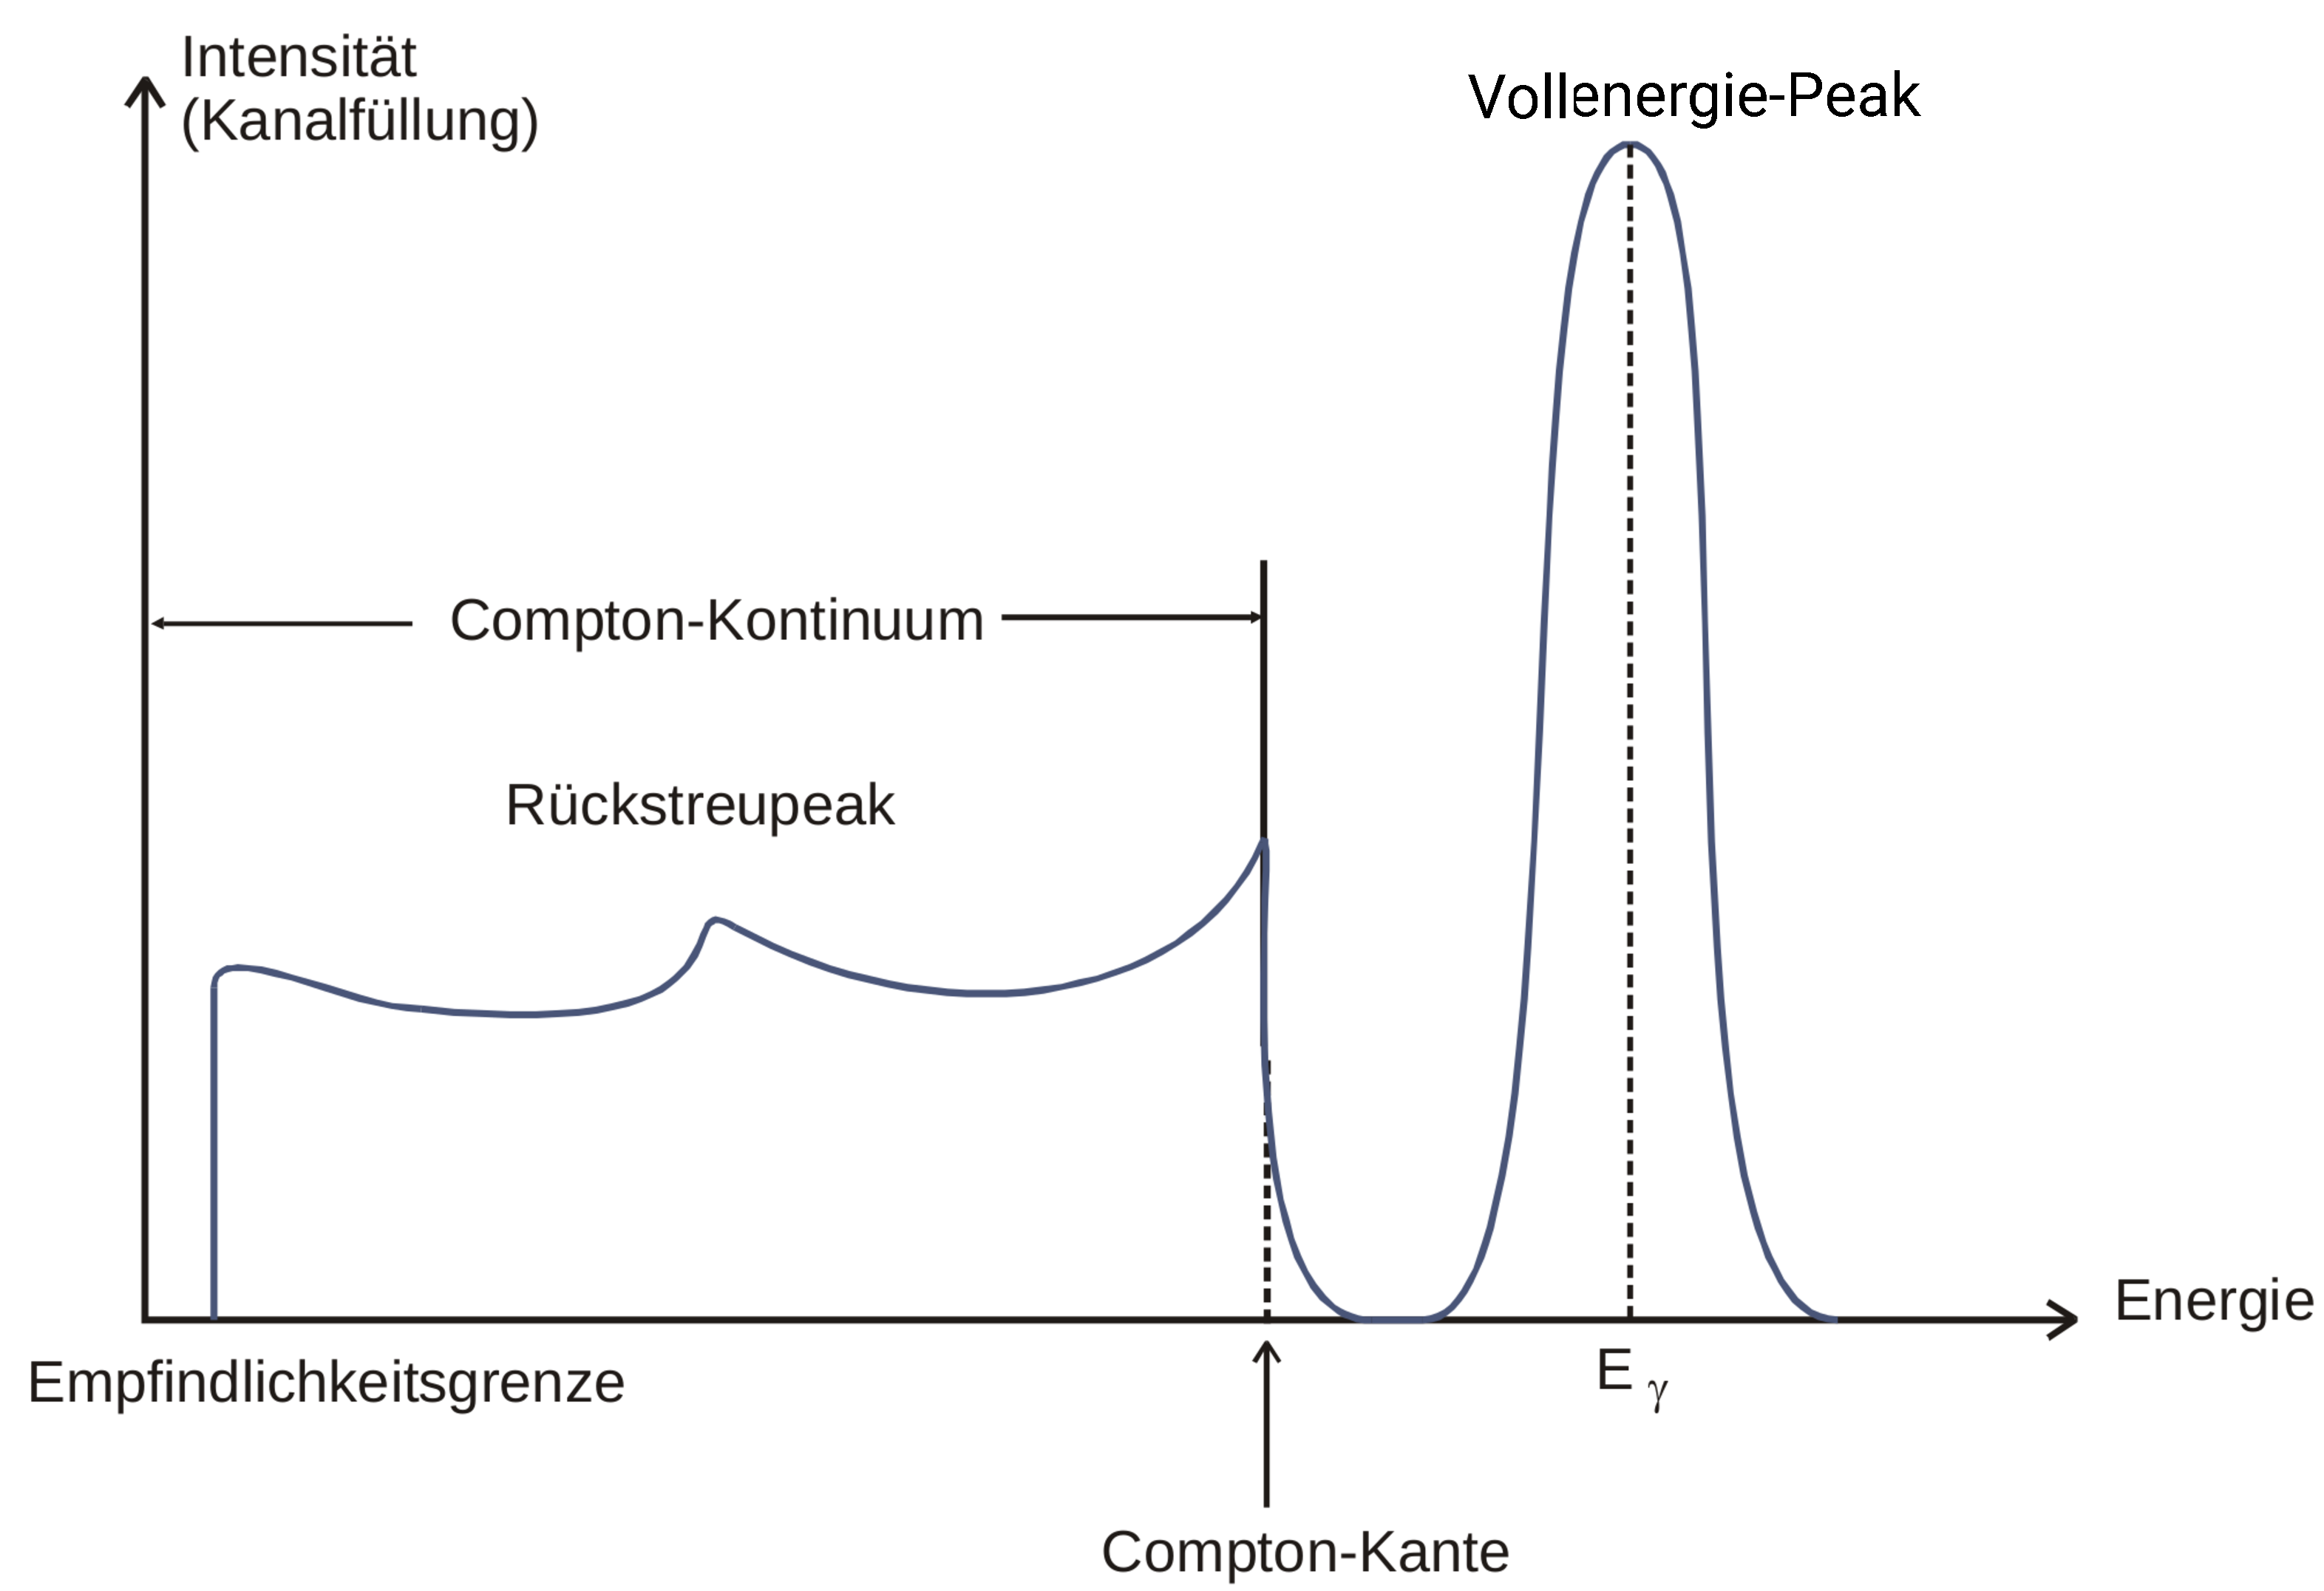
\includegraphics[width = 0.8\textwidth]{pics/example_spectrum.pdf}
\caption{Darstellung eines Energiespektrums, das mit einem Germaniumdetektor aufgenommen wird.}
\label{fig: example_spectrum}
\end{figure}